\chapter{Revisão da Literatura}
\section{Algoritmos de Regressão}

Regressão é o processo de descobrir relações entre variáveis de entrada e de saída a partir de um conjunto de dados~\cite{STULP201560}. As técnicas de regressão podem ser divididas em duas categorias principais: regressão paramétrica e não paramétrica.

A regressão paramétrica fixa uma relação funcional entre as variáveis e seu objetivo é estimar os parâmetros dessa relação. Por outro lado, a regressão não paramétrica não assume uma forma funcional específica, permitindo maior flexibilidade na modelagem de dados complexos~\cite{Angelis2023}.

\section{Algoritmos Genéticos}

Algoritmos genéticos (AGs) são uma classe de algoritmos inspirados na evolução natural, onde soluções são evoluídas ao longo de gerações para resolver problemas complexos. Eles utilizam operações como seleção, cruzamento e mutação para explorar o espaço de soluções~\cite{Angelis2023,sr_book}.

% TODO: add more information about genetic algorithms, including their application in symbolic regression.

\section{Regressão Simbólica}

Regressão simbólica é uma técnica que busca encontrar expressões matemáticas que melhor descrevem a relação entre variáveis de entrada e saída em um conjunto de dados e pode ser categorizada como uma forma de regressão não paramétrica~\cite{eggp,rEGGression}. Algoritmos considerados \textit{State of the Art} para regressão simbólica utilizam algoritmos genéticos para evoluir expressões matemáticas que representam essas relações~\cite{Olivetti_de_Fran_a_2018,sr_book,eggp}. No entanto, a regressão simbólica também pode ser implementada usando outros métodos, como redes neurais e transformadores~\cite{Angelis2023}.

\subsection{Programação Genética para Regressão Simbólica}

A programação genética utilizada na regressão simbólica evolui expressões matemáticas representadas por árvores de sintaxe abstrata (ASTs). Cada nó da árvore representa uma operação matemática (adição, subtração, multiplicação, exponenciação, etc.) e as folhas representam variáveis de entrada ou constantes. A Figura \ref{fig:ast_example} ilustra um exemplo de árvore de sintaxe abstrata para a expressão $log(x/2) + 3x$.

\begin{figure}[ht]
  \centering
  \caption{Exemplo de uma árvore de sintaxe abstrata (AST) para a expressão $log(x/2) + 3x$.}
  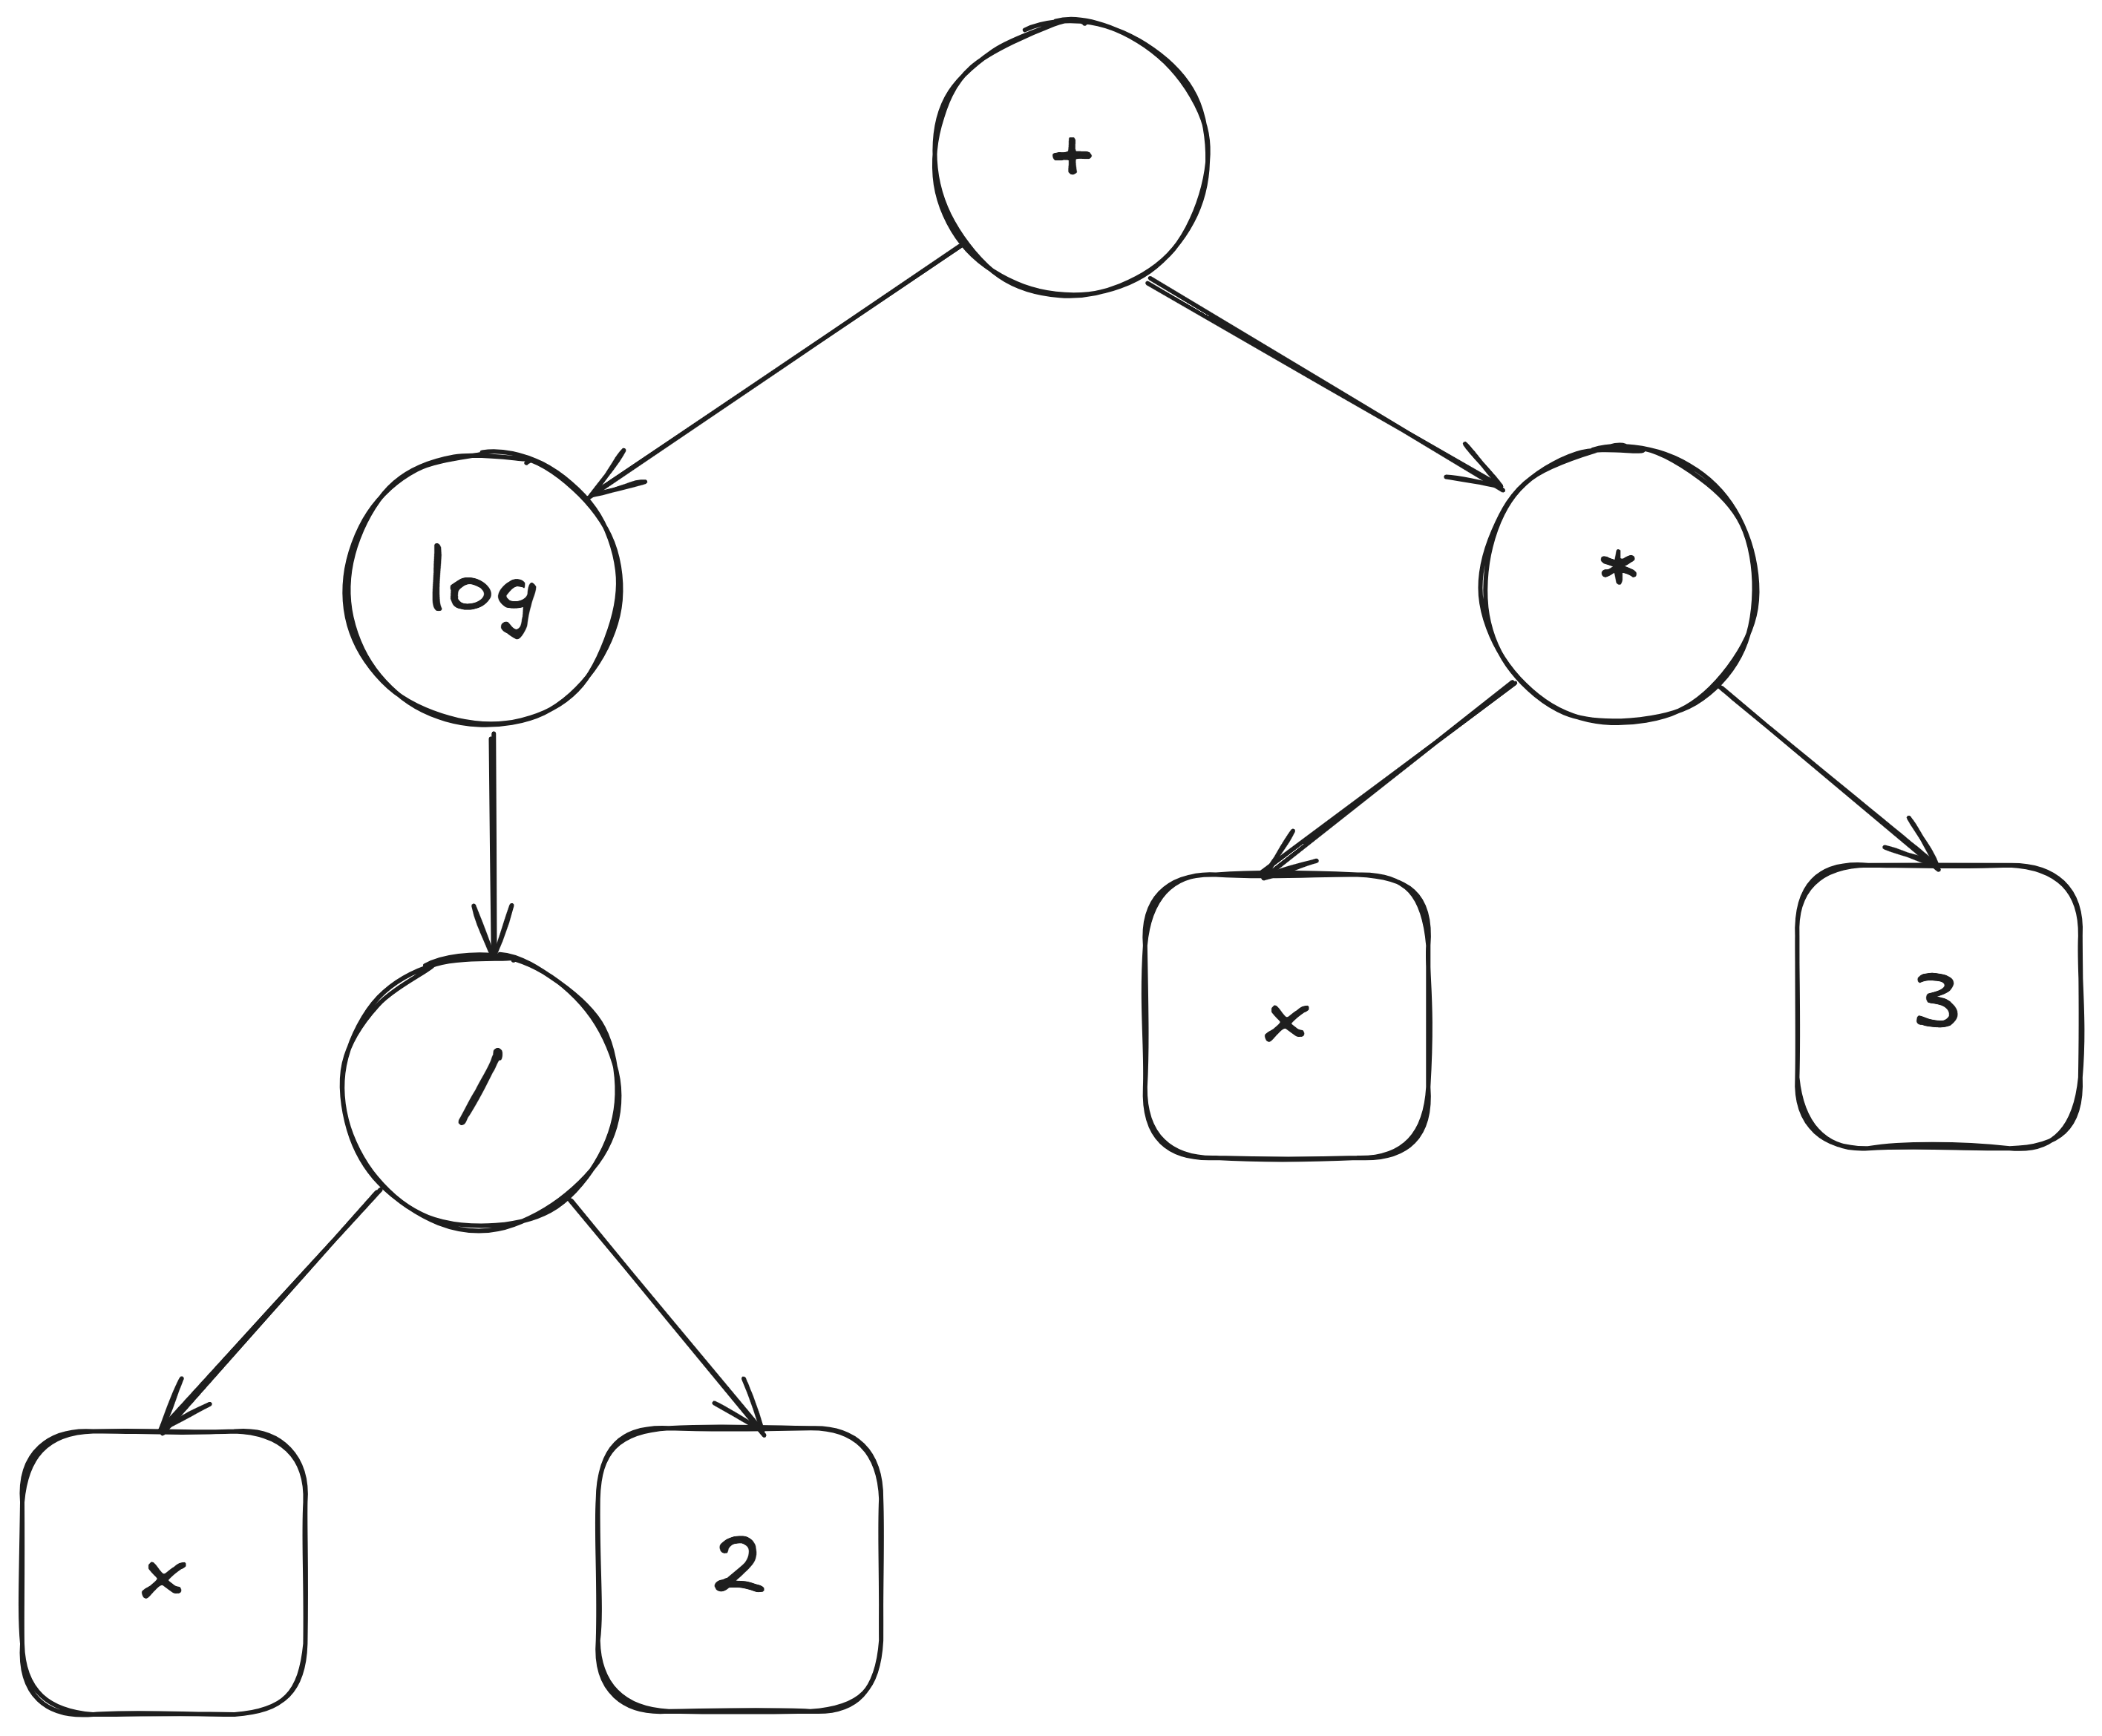
\includegraphics[width=0.5\textwidth]{images/ast_1.png}
  \label{fig:ast_example}
\end{figure}

Nós que representam operações matemáticas são representados por círculos, enquanto nós que representam variáveis de entrada ou constantes são representados por quadrados. Nós internos da árvore são chamados de não terminais, enquanto os nós folhas são chamados de terminais. O processo de busca envolve encontrar a melhor combinação de nós terminais e não terminais para minimizar a diferença entre os valores previstos pela expressão e os valores reais do conjunto de dados respeitando as restrições de complexidade e interpretabilidade da expressão~\cite{Angelis2023}.

O processo de evolução se inicia com uma população inicial de expressões aleatórias. Em cada iteração, as expressões são avaliadas com base em uma função de aptidão, que mede o quão bem cada expressão se ajusta aos dados. As melhores expressões são selecionadas para reprodução, onde passam por operações de cruzamento e mutação para gerar novas expressões que são adicionadas à nova população. Esse processo continua até que um critério de parada seja atingido. Critérios de parada comuns incluem um número máximo de gerações, obtenção da expressão ideal ou convergência da população. Comumente, uma combinação entre todos os critérios é utilizada para garantir que o processo de evolução não seja interrompido prematuramente~\cite{Angelis2023,sr_book}.

A Figura \ref{fig:ast_crossover} ilustra o processo de cruzamento entre duas expressões. Na parte superior, os indivíduos pais e, na parte inferior, os indivíduos produzidos por eles. Durante esse processo, subárvores aleatórias são selecionadas em cada expressão e trocadas entre si para criar dois novos indivíduos. Note que o cruzamento pode resultar em expressões mais complexas que os pais originais, o que pode ser controlado por meio de restrições de profundidade ou tamanho da árvore.

\begin{figure}
  \centering
  \caption{Exemplo de cruzamento entre duas expressões representadas por árvores de sintaxe abstrata (ASTs).}
  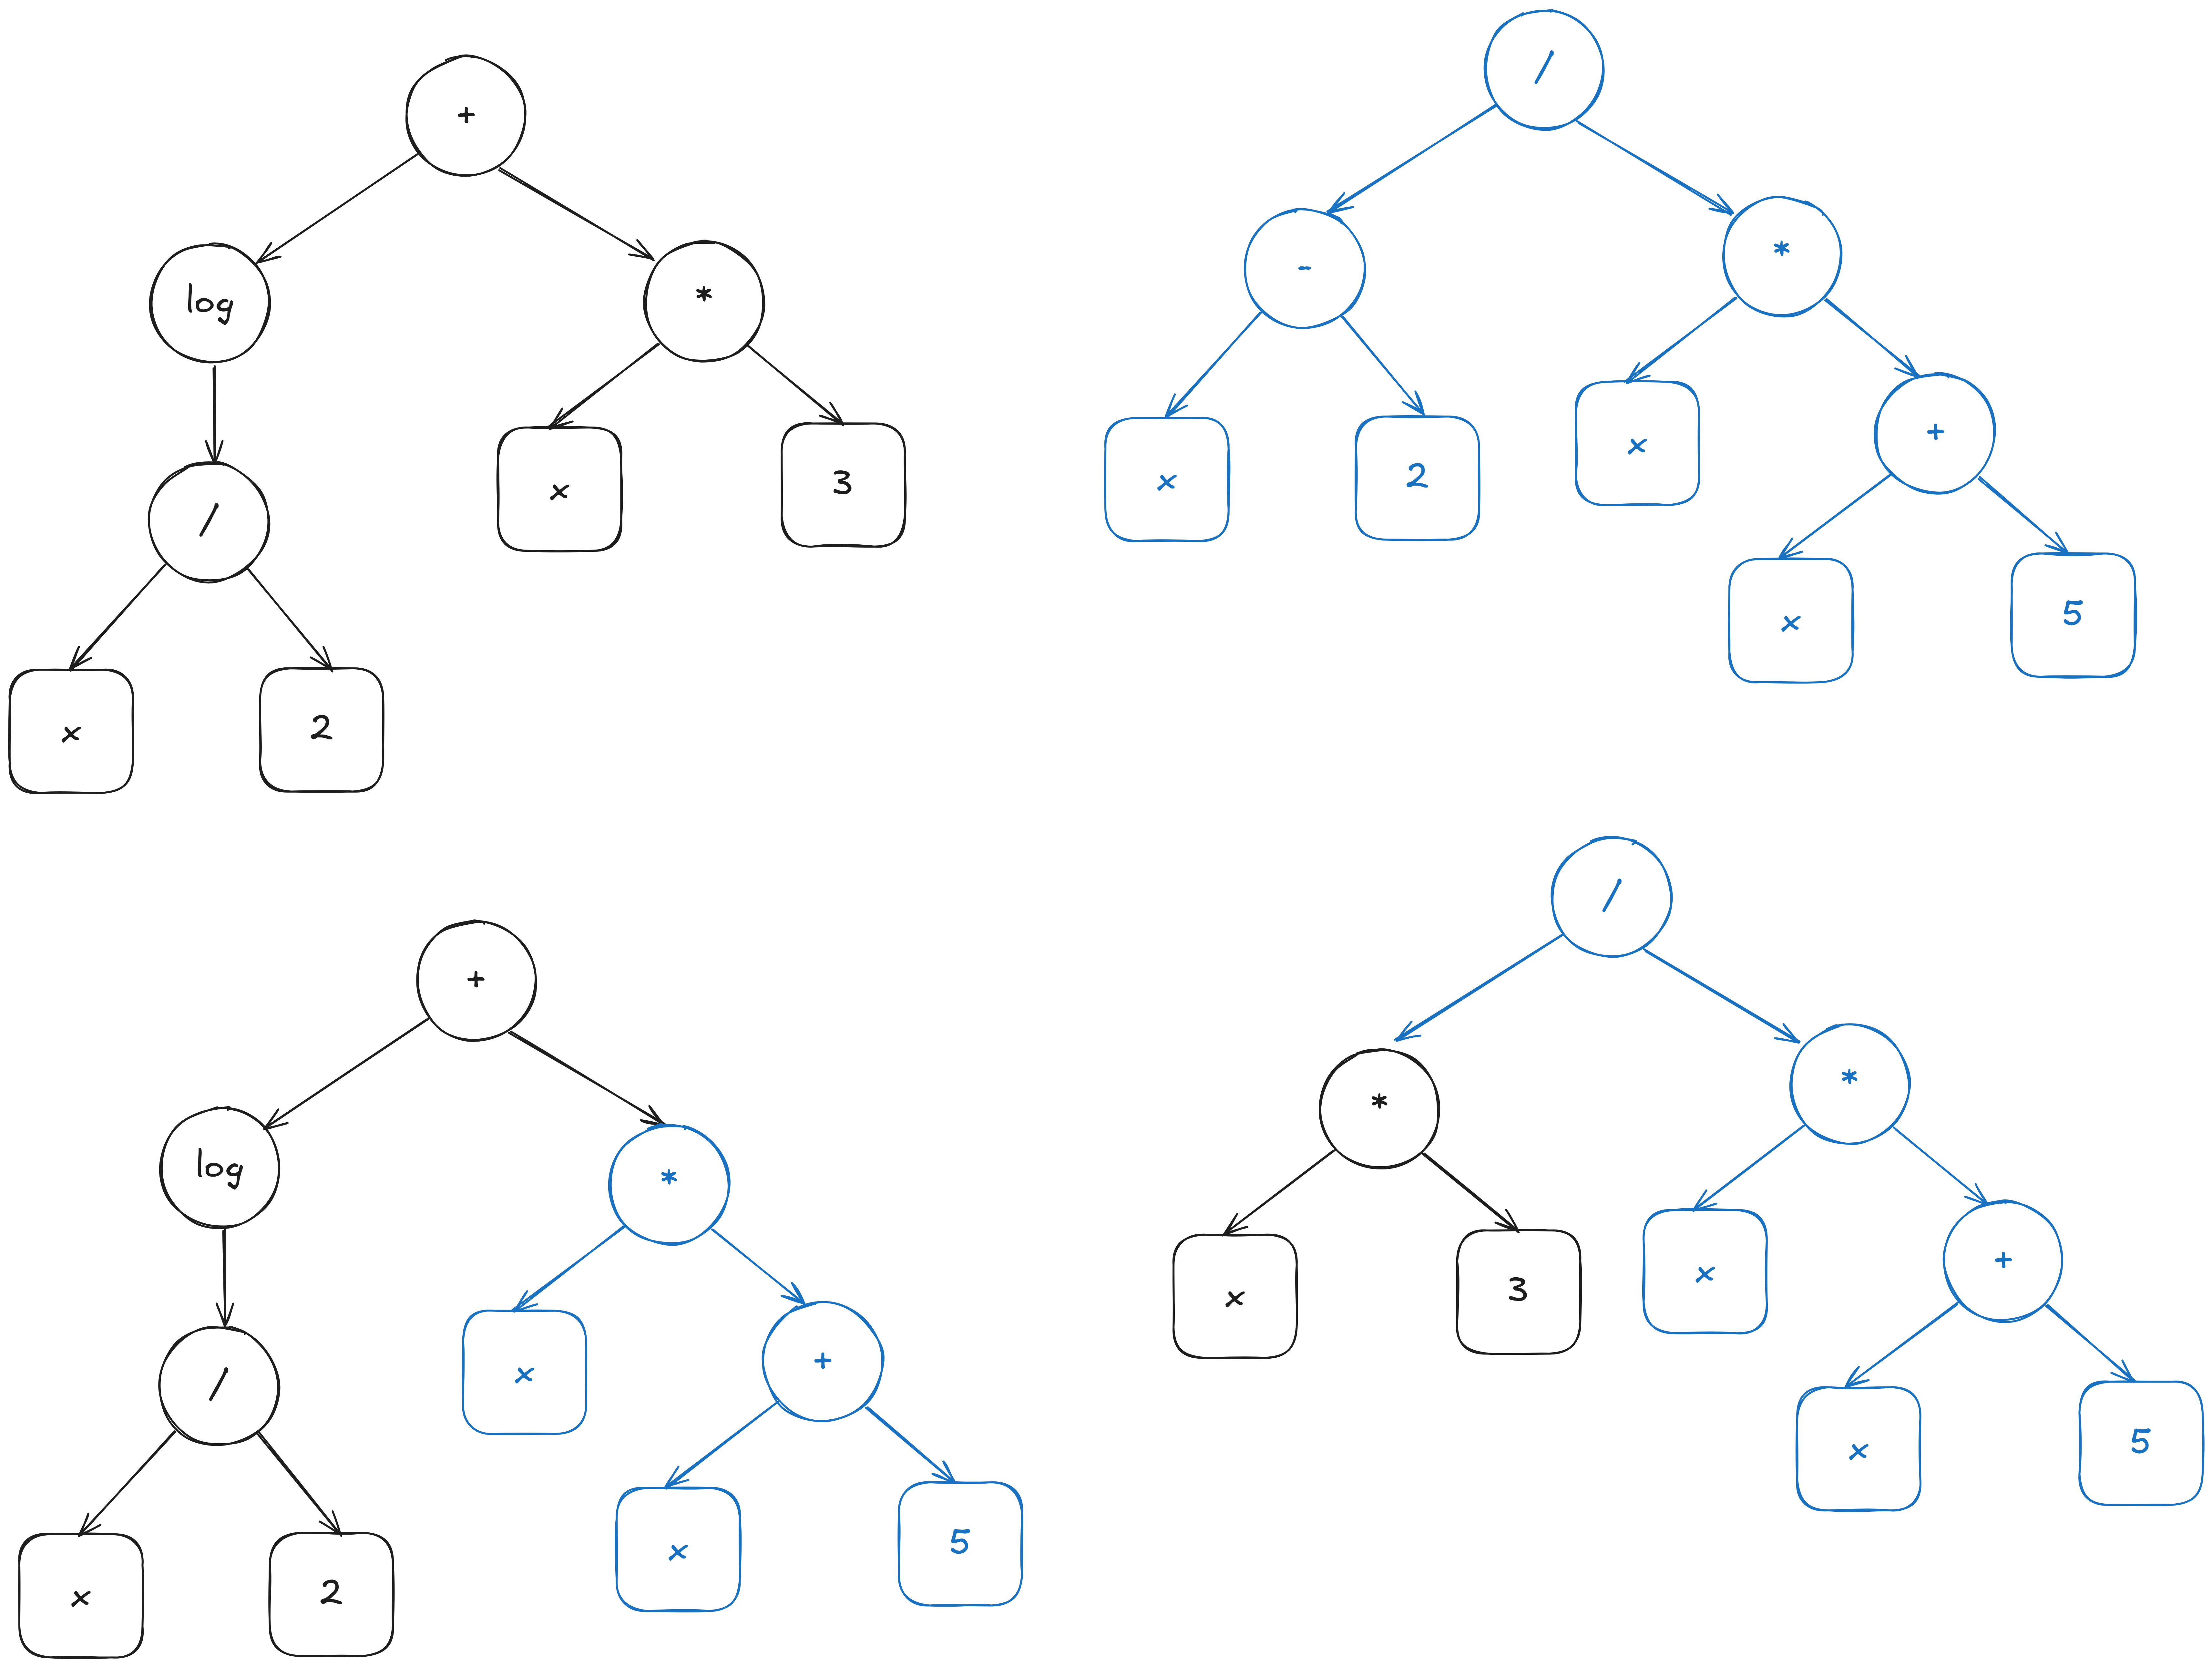
\includegraphics[width=0.8\textwidth]{images/ast_2_cross.png}
  \label{fig:ast_crossover}
\end{figure}

A Figura \ref{fig:ast_mutation} ilustra o processo de mutação, onde uma subárvore aleatória é selecionada e substituída por uma nova subárvore gerada aleatoriamente. A mutação introduz diversidade na população, ajudando a evitar a convergência prematura para soluções subótimas. Na esquerda, o indivíduo original, e na direita, o indivíduo após a mutação.

\begin{figure}
  \centering
  \caption{Exemplo de mutação em uma expressão representada por uma árvore de sintaxe abstrata (AST).}
  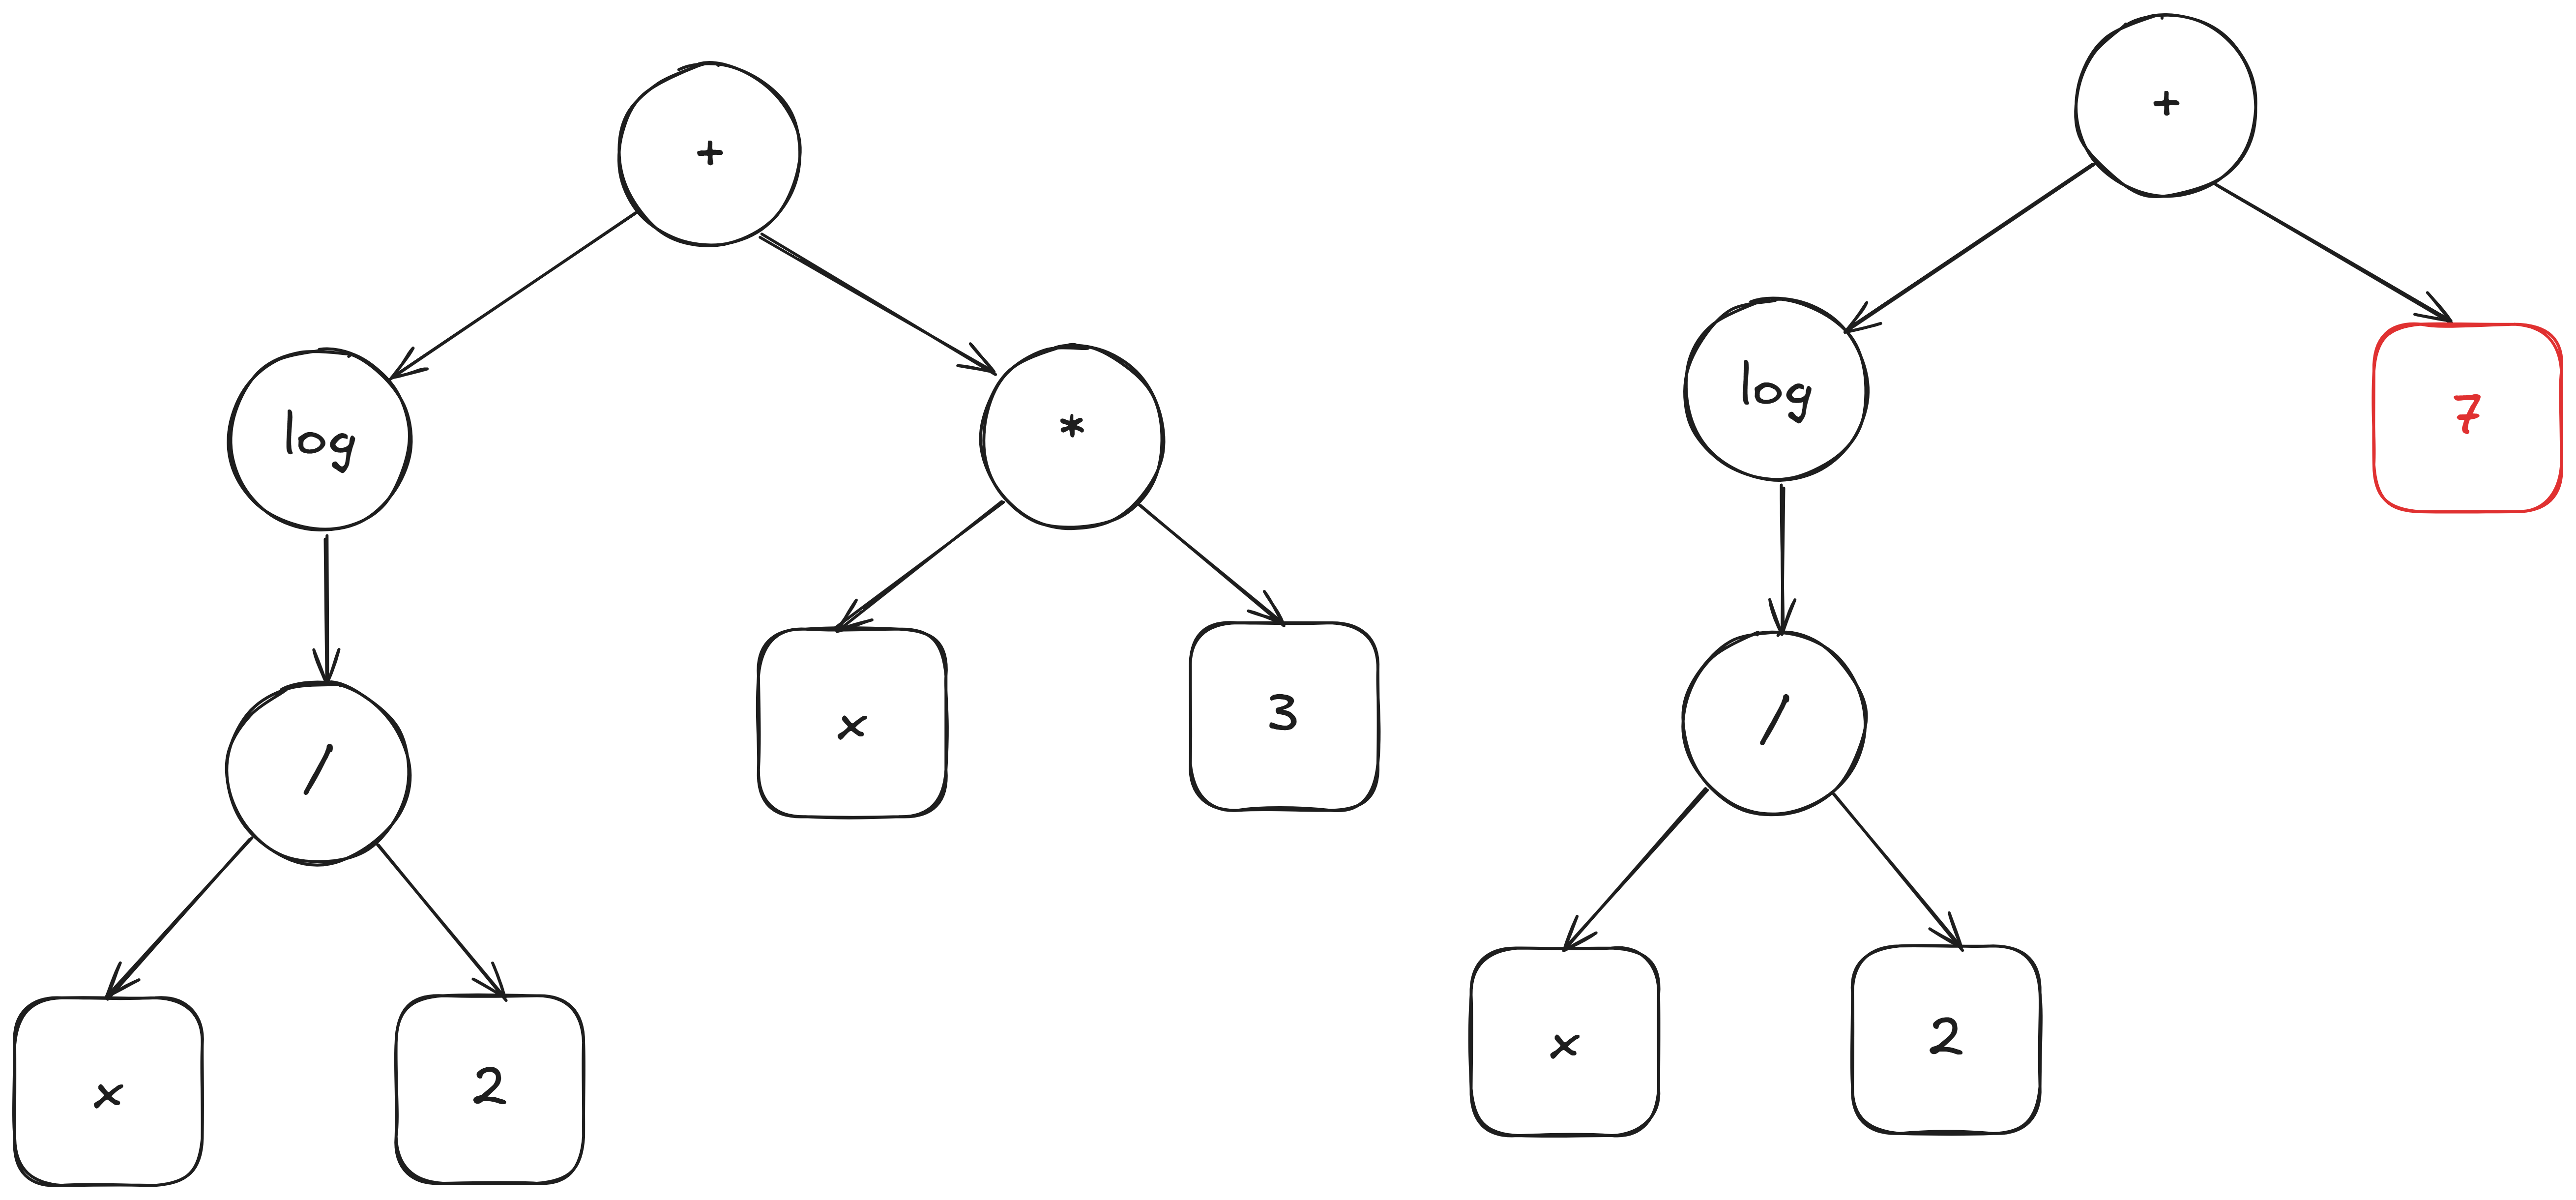
\includegraphics[width=0.5\textwidth]{images/ast_3_mutation.png}
  \label{fig:ast_mutation}
\end{figure}

É importante destacar que esse algoritmo não precisa necessariamente retornar uma única expressão. Um conjunto de expressões poder ser retornado, permitindo ao usuário escolher a que melhor se adequa às suas necessidades~\cite{Angelis2023}.

Apesar dos avanços recentes, a regressão simbólica ainda enfrenta vários desafios. A complexidade computacional decorrente do grande espaço de busca de expressões possíveis pode tornar o processo de evolução lento e ineficiente. Além disso, a interpretabilidade das expressões geradas pode ser comprometida quando elas se tornam excessivamente complexas, dificultando a compreensão por parte dos usuários finais~\cite{Angelis2023,sr_book}.

Além disso, a codificação de expressões como árvores pode levar o algoritmo de regressão a visitar expressões logicamente equivalentes várias vezes~\cite{eggp}. Por exemplo, as expressões $x + y$ e $y + x$ são logicamente iguais, mas seriam representadas por árvores diferentes. Testes empíricos indicam que apenas 40\% das expressões geradas por algoritmos genéticos para regressão simbólica são únicas~\cite{inefficiency_gp}.

\section{Saturação de igualdade para Regressão Simbólica}

Diante dos desafios enfrentados pela regressão simbólica tradicional, uma abordagem alternativa que tem ganhado destaque é o uso de grafos de igualdade (Equality Graphs - e-graphs) para representar e manipular expressões matemáticas~\cite{eggp,rEGGression}. E-graphs são estruturas de dados que armazenam múltiplas expressões equivalentes de forma compacta, permitindo a aplicação eficiente de transformações algébricas e simplificações nos indivíduos presentes no espaço de busca. Utilizando essa estrutura de dados, é possível realizar uma operação chamada de saturação de igualdade, que consiste em aplicar regras de reescrita para gerar todas as expressões logicamente equivalentes a uma dada expressão inicial.

\subsection{Grafos de Igualdade}

Grafos de igualdade são estruturas de dados que representam expressões matemáticas e suas equivalências de maneira eficiente. Elementos matemáticos são representadas por e-nodes, enquanto classes de expressões equivalentes são representadas por e-classes. Cada e-class contém um conjunto de e-nodes que representam diferentes formas de expressar a mesma expressão matemática. Cada e-node aponta para e-classes filhas, que representam os operandos da operação matemática representada pelo e-node.

A Figura \ref{fig:egraph_example} ilustra um grafo de igualdade. Note que as expressões $2x$ e $x + x$ pertencem à mesma e-class, uma vez que são logicamente equivalentes. A implementação de e-graphs utiliza uma estrutura union-find para gerenciar a união de e-classes quando novas equivalências são descobertas durante o processo de saturação~\cite{eggp}. Uma e-class armazena uma lista de e-nodes que pertencem a ela, uma lista de e-nodes pais (e-nodes que possuem essa e-class como filha) e demais informações auxiliares para otimizar operações de busca e união.

\begin{figure}
  \centering
  \caption{Exemplo de um grafo de igualdade, adaptado de~\cite{eggp}.}
  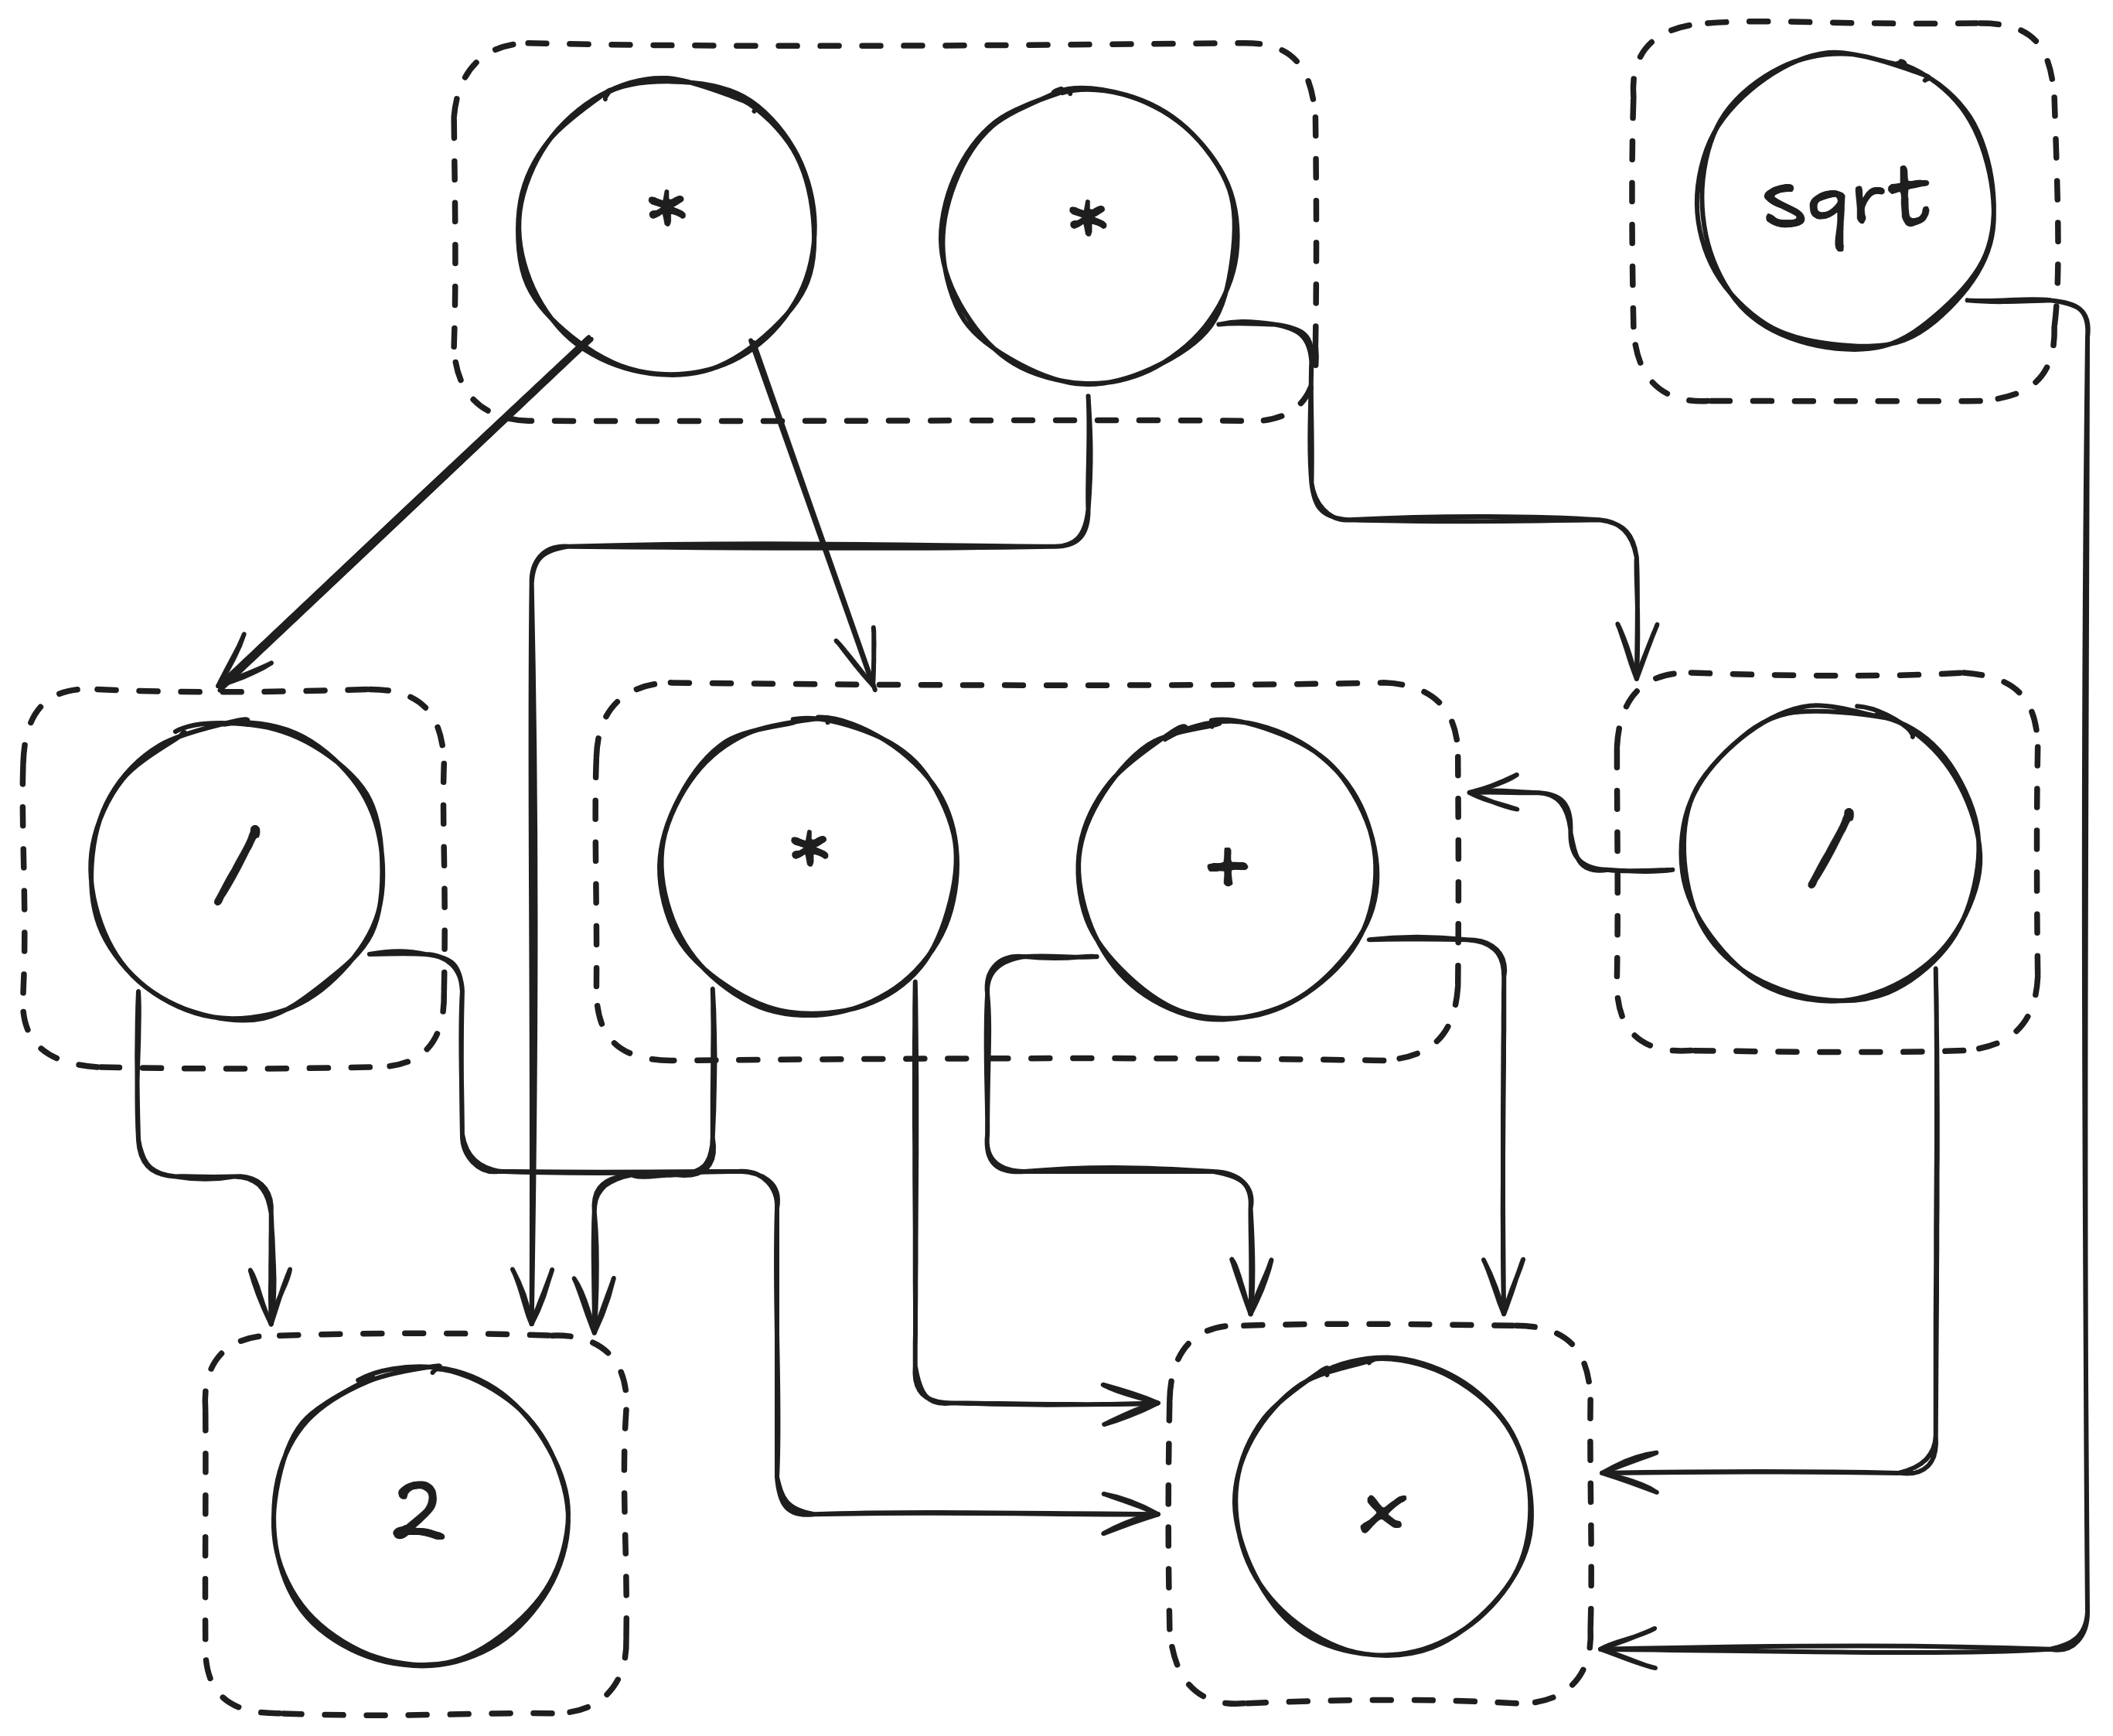
\includegraphics[width=0.7\textwidth]{images/egraph.png}
  \label{fig:egraph_example}
\end{figure}
